%*****************************************
\chapter{Methods}
\label{ch:methods}
%*****************************************
\section{Model description of MPI-ESM}

%\renewcommand{\thefigure}{A\arabic{figure}}
\counterwithin{figure}{chapter}
\counterwithin{table}{chapter}
%preamble: 
%\paragraph{Model components} 
The \acf{MPI-ESM} 
consists of coupled general circulation models of the atmosphere \acs{ECHAM}6 \citep{Stevens2013} and ocean \acs{MPIOM} \citep{Jungclaus2013} as well as subsystem models for vegetation on land JSBACH \citep{Reick2013} and for marine biogeochemistry \acs{HAMOCC} \citep{Ilyina2013}. The large ensemble simulations are based on \acs{MPI-ESM} version 1.1.00p2 \footnote[1]{full source code: \url{https://code.zmaw.de/projects/mpi-esm/repository/show/tags/mpiesm-1.1.00p2}} with a low-resolution configuration. Since the atmospheric pCO$_2$ levels are prescribed, terrestrial carbon cycle from the land component JSBACH and oceanic carbon cycle from \acs{HAMOCC} do not interact (\autoref{fig:MPIESM}). The full \acf{ESM} \citep{Giorgetta2013} as well as its components have been described and evaluated in detail by the given references. In the following subsections, I give an overview about the implemented processes affecting internal variability of the oceanic carbon cycle.



%The Max-Planck-Institute for Meteorology Earth System Model (MPI-ESM) version 1.1.00p2 \footnote[1]{full source code: \url{https://code.zmaw.de/projects/mpi-esm/repository/show/tags/mpiesm-1.1.00p2}} with a low-resolution configuration is used for the large ensemble simulations \citep{Giorgetta2013}. The atmosphere component ECHAM6.3 runs on a T63 grid, corresponding to 1.9$^\circ$ horizontal resolution, with 47 vertical layers up to 0.01 hPa \citep{Stevens2013}. The ocean component MPI Ocean Model (MPIOM) has a horizontal resolution of 1.5$^\circ$ on average and 40 fixed-depth vertical levels \citep{Jungclaus2013}. The Hamburg Ocean Carbon Cycle Model (HAMOCC) represents the ocean biogeochemistry component (fig. \ref{fig:HAMOCC}) \citep{Ilyina2013}. Since there is no biogeochemical riverine exchange, terrestrial carbon cycle from JSBACH \citep{Reick2013} and oceanic carbon cycle do not interact (fig. \ref{fig:MPIESM}). 

\begin{figure}[h!]
	\centering 
	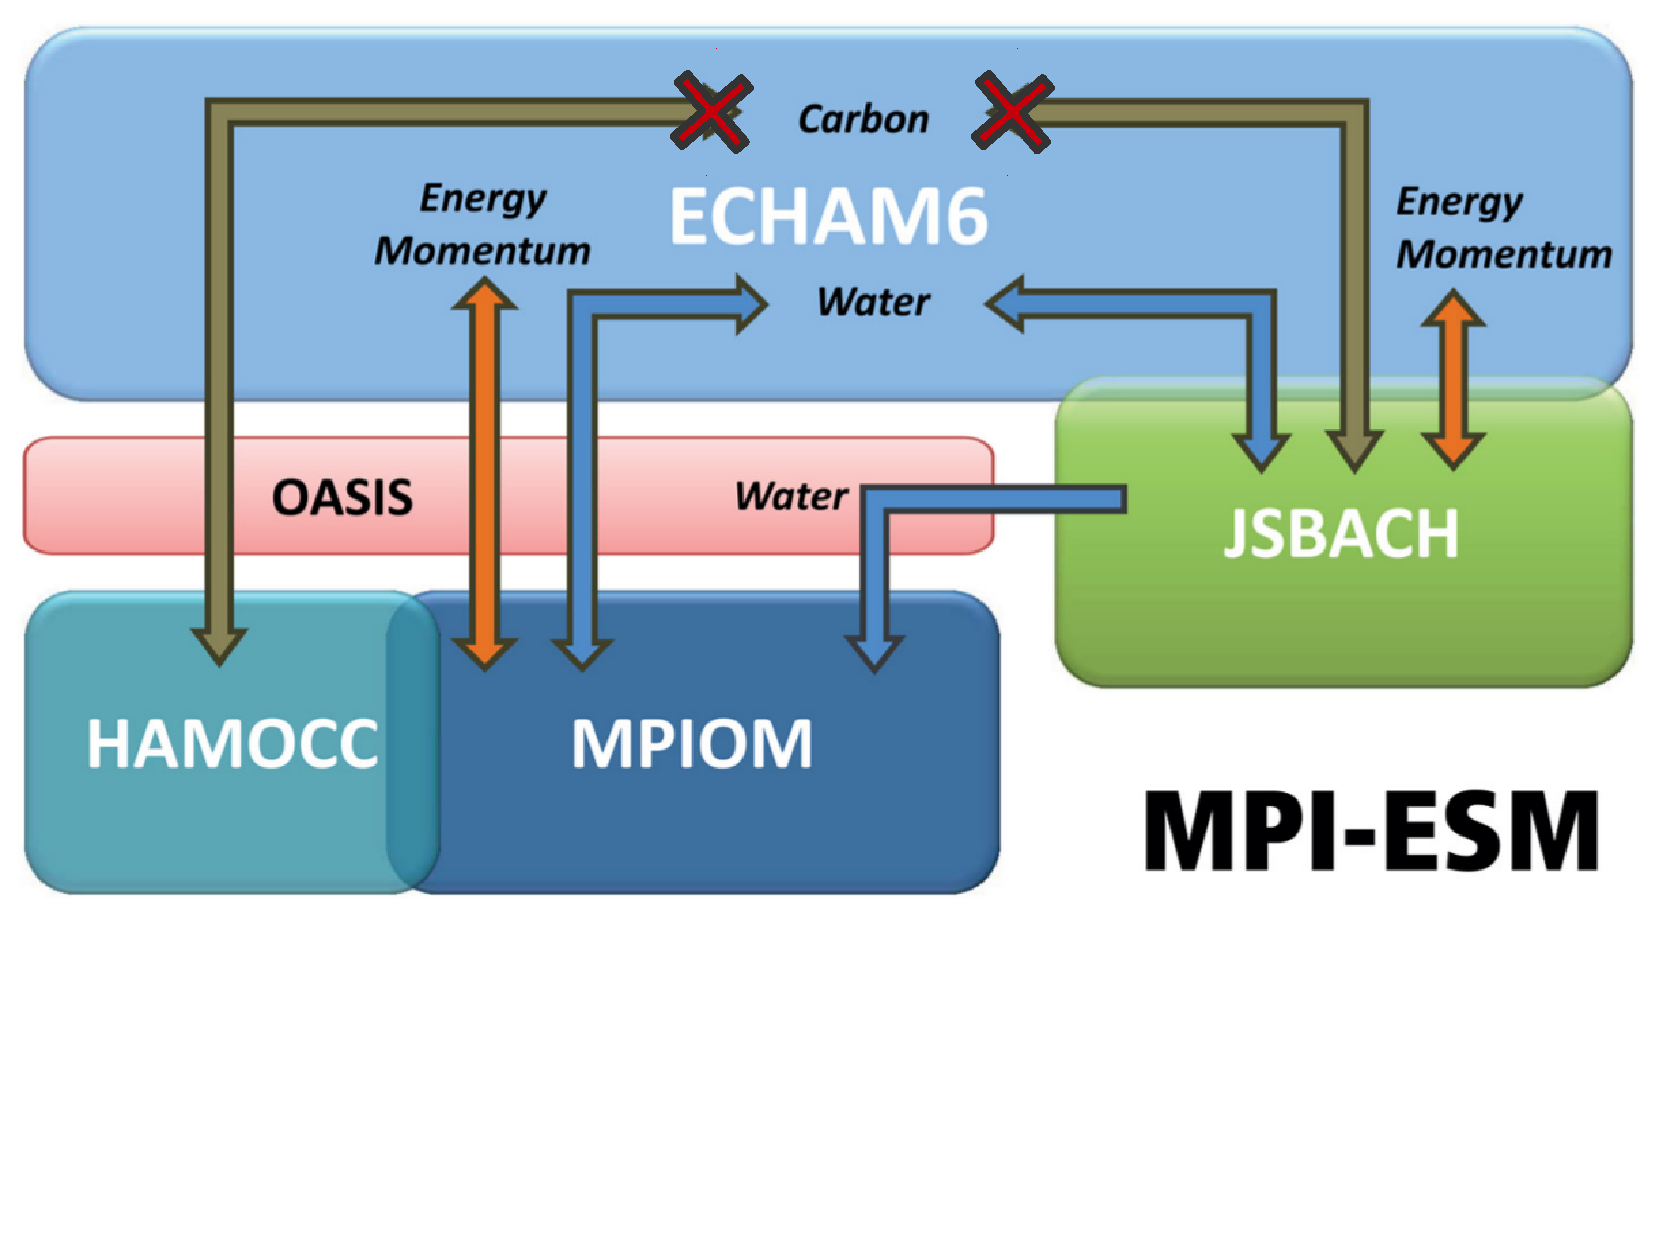
\includegraphics[scale=.42,trim=0cm 5.87cm 0cm 0cm,clip]{MPIESM.pdf}
	\caption{Schematic overview on the different components in \ac{MPI-ESM} with prescribed atmospheric partial pressure pCO$_{\text{2,atm}}$ \citep{Giorgetta2013}}
	\label{fig:MPIESM}
\end{figure}

%\subparagraph{Note: I briefly explain how processes affecting the carbon cycle/my study are implemented and subject to internal variability}


\subsection{ECHAM}
\acs{ECHAM} is an general circulation model for the atmosphere. \acs{ECHAM} has an sea-air gas exchange interface with \acs{HAMOCC} and furthermore couples water, energy and momentum fluxes with \acs{MPIOM}. 
The atmosphere component \acs{ECHAM}6.3 runs on a T63 grid, corresponding to 1.9$^\circ$ horizontal resolution, with 47 vertical layers up to 0.01 hPa \citep{Stevens2013}. 
This high vertical resolution and atmospheric height allows to model jets originating in the tropopause. Those jets define the position and strength of the westerly winds in the Southern hemisphere. %In \acs{ECHAM} extra-tropical jets are slightly shifted to lower latitudes \citep{Stevens2013} which seems to be a common atmospheric modeling challenge \citep{Kidston2010}.
Changes in \acs{ECHAM} with regard to \acs{CMIP5} version in \cite{Stevens2013} are described in \cite{Bittner2016}. They majorly include the new radiation code of \acs{ECHAM}6.3.% which leads to small changes in the temperature fields.  


\subsection{MPIOM}
\label{sec:mpiom}
%\subparagraph{relevant MPIOM info: upwelling/advection/mixing}
The \ac{MPIOM} is an ocean general circulation model (OGCM) with a horizontal resolution of 1.5$^\circ$ on average on the Arakawa C-grid, 40 fixed-depth vertical levels on a realistic topography and with a free surface \citep{Jungclaus2013}.  %All biogeochemical and physical tracers except for opal and calcite shells are advected by the Navier-Stokes equations with Boussinesq-approximation \citep{Marsland2003}. 
%In areas of large scale upwelling - such as the Southern Ocean - those tracers are advected to the ocean surface. Those carbon-rich waters then equilibrate with atmospheric pCO$_2$. Upwelling processes are largely driven by divergence due to winds. Strong ocean currents lead to eddies which additionally mix the water column horizontally and vertically. 
The spatial resolution of 1.5$^\circ$ translated to a grid cell length of $\sim$150 km at the northern edge of the Southern Ocean at 30$^\circ$S and $\sim$40 km in Antarctic coastal waters. %These length scales are too small to resolve eddies, so they are parametrized by the GM-scheme \citep{Gent1995}. 
Eddies are parametrized by the GM-scheme \citep{Gent1995}. Therefore, the vertical mixing and diffusion based on Richardson-number dependent formulation is important for vertical gradients \citep{Pacanowski1981}. Tracers are advected by the Navier-Stokes equations with Boussinesq-approximation.%The impact of eddies on the carbon cycle, especially in the Southern Ocean, is under current research \citep{Lauderdale2013,Dufour2013,Gnanadesikan2015}.

The \ac{MLD} is calculated by a potential density criterion where the difference between the sea-surface density and the lower end of the mixed-layer is 0.125 kg m$^{-3}$ \citep{Jungclaus2013}. 




\subsection{HAMOCC}
\label{sec:HAMOCC}
%\subparagraph{HAMOCC coupling} 
%HAMOCC is coupled to ECHAM6 for exchange of atmoshperic gases, precipitation and energy, e.g. heat as radiation and mechanical energy as wind stress. The required state variables required for HAMOCC, such as sea-ice cover, temperature T, salinity S and advective velocities $\vec{v}$, are provided from MPIOM. 
The \ac{HAMOCC} is a global marine carbon cycle model which simulates oceanic carbon and nutrient cycles \citep{Maier-Reimer1984,Maier-Reimer1993,Six1996}. As a subsytem in the ocean, biogeochemical tracers except for opal and calcite shells are advected by \acs{MPIOM}. \acs{HAMOCC} aims to reproduce distributions of biogeochemical parameters over various timescales from seasons to millenia without regional tuning or temporal adjustments towards observations \citep{Ilyina2013}. This includes processes on three compartments: sea-air interaction at the sea surface, biogeochemistry of the water column and sediment biogeochemistry (\autoref{fig:HAMOCC}). The \acs{HAMOCC} model version for the large ensemble is identical to the one used in \acs{CMIP5} which is analyzed in detail in \cite{Ilyina2013}. In the following subsection, I will only give an overview about the implementation of the most relevant processes for the variability on decadal and shorter timescales.\newline

\begin{figure}[h!]
	\centering
	\includegraphics[scale=.60,page=2,trim=2.8cm 1.3cm 3.4cm .6cm,clip]{HAMOCC_scheme_feedback_new.pdf}
	\caption{Schematic overview of the global ocean biogeochemistry model \acs{HAMOCC} \citep{Ilyina2013} which is coupled to the atmospheric model component \acs{ECHAM} and the ocean model \acs{MPIOM}. The ocean model provides state variables of physical oceanography, i.e. ice cover, temperature (T), salinity (S) and the advective velocities ($\bar{v}$).
	 The water column holds tracers of gases, i.e. oxygen (O$_2$), nitrogen (N$_2$), laughing gas (N$_2$O), and dimethyl sulfide (DMS); nutrients, i.e. iron (Fe), phosphate (PO$_4$), nitrate (NO$_3$) and silicic acid Si(OH)$_4$; and tracers of carbonate chemistry, \ie \acf{DIC} and alkalinity (Alk). Photosynthesis converts \ac{DIC} and nutrients to \acf{DOC}, which produces calcium carbonate (CaCO$_3$) or opal shells.}
	\label{fig:HAMOCC}
\end{figure}

The carbonate system determines pCO$_{\text{2,ocean}}$ \citep{Maier-Reimer1993}. Dissolved inorganic carbon and alkalinity are directly calculated as prognostic tracers from which other tracers derived. When pCO$_{\text{2,atm}}$ reacts with seawater, the carbonate chemistry evaluates pCO$_{\text{2,ocean}}$ based on the law of mass action formulae depending on temperature (calculated according to \cite{Weiss1974}), salinity, \acs{DIC} and alkalinity.%\newline

%\paragraph{CO$_2$ flux description}
The CO$_2$ flux calculation implemented in the model follows an empirical relationship under the conceptual one-layer ocean-sided stagnant film model with gas transfer velocity $k_w$ \citep{Wanninkhof1992}: 
\begin{align}
\text{CO}_2\text{flux} &= (1-f)k_w \Delta \text{pCO}_2 \label{eq:HAMOCC}\\
				k_w &= 0.31 u_{10}^2(\text{Sc(T)}/660)^{-\frac{1}{2}} \notag \\
				\Delta \text{pCO}_2 &= \text{pCO}_{2\text{,ocean}} - \text{pCO}_{2\text{,atm}} \text{,} \notag
\end{align}
where $f$ is the the sea-ice fraction of the grid cell, $u_{10}$ is the wind speed at 10 m height, $\text{Sc}$ is the temperature-dependent Schmidt number, 660 is the Schmidt number of CO$_2$ in seawater at 20$^\circ$C and $\Delta \text{pCO}_2$ is the difference between the partial pressure of CO$_2$ in the atmosphere and the ocean, so positive values of sea-air CO$_2$ flux represent a net flux from the ocean to the atmosphere. %The potential partial pressure of CO$_2$ in water pCO$_{2\text{,ocean}}$ is solubility-dependent by Henry's law and calculated according to \citep{Weiss1974}.\newline %The solubility is primarily temperature sensitive. Ocean warming decreases solubility, whereas cooling increases it. Therefore saturated surface waters outgas when heated - a process referred to as the solubility pump of carbon \citep{VolkHoffert1985}.\newline

%\paragraph{CO$_2$ flux variability}
%The disequilibrium $\Delta \text{pCO}_\text{2}$ drives CO$_2$ flux variability by setting the direction of CO$_2$ flux. As pCO$_{2\text{,atm}}$ is prescribed in the \acs{MPI-ESM LE}, changes in pCO$_{2\text{,ocean}}$ are the main driver of CO$_2$ flux variability. The carbonate chemistry directly relates pCO$_{2\text{,ocean}}$ to surface dissolved inorganic carbon (\acs{DIC}). Besides CO$_2$ flux, surface \acs{DIC} is mainly changed by biology (see below) and advection (see section \ref{sec:mpiom}).\newline


%\paragraph{Biology}
In the euphotic zone upto a depth of 90m, phytoplankton converts inorganic nutrients, e.g. phosphate (PO$_4$), nitrate (NO$_3$), iron (Fe) and \acs{DIC} to organic matter by photosynthesis. %The predator-prey relationship in \acs{HAMOCC} follows an extended \acs{NPZD} model \citep{Six1996}. Phytoplankton proliferate from nutrient consumption.  Zooplankton consume phytoplankton, while detritus forms as opal and calcium carbonate shells and sinks down the water column, a process referred to as the biological pump \citep{VolkHoffert1985}. While detritus sinks to the ocean floor, it partly remineralizes and gives rise to nutrient and \acs{DIC} concentrations, which can lead to outgassing once they are advected to the surface. 
The biological pump \citep{VolkHoffert1985} is implemented based on an extended \acs{NPZD}-type ecosystem formulation \citep{Six1996}. Phytoplankton growth is co-limited by nutrients (phosphate, nitrate and iron), temperature and light: Phytoplankton is parametrized by bulk phytoplankton, which mimics the combined growth of diatoms, coccolithophores and dinoflagellates under exponentially increasing optimum growth rate temperatures \citep{Eppley1972}. 
Phytoplankton growth depends linearly on the availability of light, without saturation for stronger irradiance. The temperature-irradiance dependence is combined by a limitation function in \cite{Smith1936} (\autoref{fig:lighttemplimf}). 
Michaelis-Menten kinetics describe the nutrient limitation of the maximum phytoplankton growth rate with a half-saturation constant \citep{MichaelisMenten1913}. The limiting role of nutrients is described by the nutrient availability factor that multiplies with the average growth rate of phytoplankton. 
The macro-nutrient iron is modeled by iron-relaxation from lignans. Iron enters the water column via a monthly dust input climatology, is used in photosynthesis and released in remineralization.%\newline



%\paragraph{Variability in biology due to changing physical conditions}


%\paragraph{Misc with low impact on carbon variability: chemistry and sediment}
%Other processes in a biogeochemical model act on longer timescales or small amplitude and hence lack a strong variability signal in the carbon cycle. 



There are two different falling detritus: opal producing, if silicate is available or else calcium carbonate producing. %Calcification then changes the alkalinity and carbon budget.

Once detritus reach the the ocean floor, particulate matter enters the sediment and finally the burial layer. At the upper boundary of the sediment all tracers are in exchange with the sediment via pore water exchange \citep{Heinze1999}. 

%%%%%%%%%%%%%%%%%%
%\section{Internally varying processes corresponding to CO$_2$ flux}
%potentially all into ch 3 or ch 4
%from mpiom
%unwichtig In areas of large scale upwelling - such as the Southern Ocean - those tracers are advected to the ocean surface. Those carbon-rich waters then equilibrate with atmospheric pCO$_2$. Upwelling processes are largely driven by divergence due to winds. Strong ocean currents lead to eddies which additionally mix the water column horizontally and vertically.

%from hamocc
% ch4: The solubility of pCO$_{\text{2,ocean}}$ is primarily temperature sensitive. Warmer oceans such as in the the tropics have lower solubility than cooler high-latitude oceans - a process referred to as the solubility pump of carbon \citep{VolkHoffert1985}. Likewise, CO$_2$-equilibrated waters outgas when warmed and take up CO$_2$ when cooled.

% ch4 The disequilibrium $\Delta \text{pCO}_\text{2}$ drives CO$_2$ flux variability by setting the direction of CO$_2$ flux. 
%unwichtigAs pCO$_{2\text{,atm}}$ is prescribed in the \acs{MPI-ESM LE}, changes in pCO$_{2\text{,ocean}}$ are the main driver of CO$_2$ flux variability. 
%The carbonate chemistry directly relates pCO$_{2\text{,ocean}}$ to surface dissolved inorganic carbon (\acs{DIC}) and alkalinity. Besides CO$_2$ flux, surface \acs{DIC} and alkalinity are mainly changed by biology (see below) and advection (see section \ref{sec:mpiom}).

% ch4 Biological processes are strongly dependent on physical properties of the ocean circulation. Mixing can change the nutrient distributions, when remineralized nutrients from the deep ocean mix into the euphotic zone. Mixing can also pull the standing stock of phytoplankton deeper into the ocean where less light is available which inhibits growth. Changes in sea surface temperature also directly affect phytoplankton growth. 

%While detritus sinks to the ocean floor, it partly remineralizes and gives rise to nutrient and \acs{DIC} concentrations, which can lead to outgassing once they are advected to the surface. 

%Also the processes in the atmosphere alter biological production: Cloud-cover reduces photosynthetic active radiation and freshwater fluxes dilute nutrient concentrations.\newline

%As the Southern Ocean is rather deep and my analysis does not focus on the shelf areas, I neglect the slow sedimentary processes. 
%\clearpage

\section{Large ensemble simulations}
\label{sec:PICLE}
%\paragraph{Perturbed initial conditions large ensembles}
Large ensemble simulations are a novel tool to investigate model internal variability. "Climate variability refers to variations in the mean state (...), which may be due to natural internal processes within the climate system (internal variability), or to variations in natural or anthropogenic external forcing (external variability)" \citep{IPCC}. The variability in observations is impossible to separate, if - like in the case of pCO$_{\text{2,ocean}}$ - no long-lasting direct measurement records exist.
Although modeled internal variability is not equivalent to observed internal variability, we can learn about the random variations of natural processes.

By iterating a climate simulation with an identical forcing and model code but slightly perturbed initial conditions, single ensemble members will be exposed to the same process implementations. The interplay of those at a stochastically random level lets each realization evolve in a unique way while still being bound to a common forced signal following the external forcing. Perturbed initial conditions large ensemble simulations allow to distinguish a signal into a force signal which is the average signal across all ensemble members, and the residual which modulates the signal around the forced signal due to internal variability [\cite{McKinley2016}; {\color{RoyalBlue}2017}]: 
\[ \text{signal}=\text{forced signal}+\text{internal variability}.\]
%This residual is caused by internal variability and in the case of the Southern Ocean closely linked to the Southern Annular Mode (SAM).

As running large ensembles simulation comes with high computational costs, this area of climate modeling research is still more recent. There are only a few datasets available and published papers are still rare, \eg \cite{Deser2012,Thompson2015,Lovenduski2016,Krumhardt2017, Kay2015,McKinley2016,ilyinaletter2016,Bittner2016,Hedemann2017,Rodgers2015}.\newline 
%\paragraph{MPI-ESM Large Ensemble} 

The \acs{MPI-ESM LE} contains 100 simulations under historical \acs{CMIP5} forcing from 1850 to 2005. %and is extended under \ac{RCP} 4.5 scenario until 2100, so t
The forcing includes volcano eruptions from the historical period and solar cycles. Anthropogenic forcings include well-mixed greenhouse gases, anthropogenic sulphate aerosols and land-use change. Atmospheric pCO$_2$ levels are prescribed according to the \acs{CMIP5} protocol \citep{Taylor2012}. The carbon cycle is not coupled, so effects of changes in the terrestrial or oceanic carbon sink are not reflected in the atmospheric pCO$_{\text{2,atm}}$. 

Ensemble members differ through starting from different year of the pre-industrial control simulation, so ocean and atmosphere have slightly different initial conditions in each run. This was achieved by branching off ensemble members from a 2000-year pre-industrial control run after roughly 50 years, when the historical forcing sets it.\newline %atmospheric pCO$_2$ levels were increased. 

%The historical part of \acs{MPI-ESM} from 1850 to 2005 was calculated at the Swiss National Supercomputing Centre (CSCS), the \acs{RCP} extension on the supercomputer Mistral at the German climate research center (DKRZ). The model and run script were compatible, however different hardware and compilers might lead to changes in variability distributions. Therefore, I restrict the analysis of decadal internal variability to the time-frame between 1980, the beginning of the observational dataset and 2005.\newline
 

%MPI-ESM LE data already provided data to a few MPI-M publications, e.g. \citep{Bittner2016},\citep{Hedemann2017}.

%\paragraph{Other large ensemble simulations} 



\acs{NCAR}'s \ac{CESM} \acs{LE} \citep{Kay2015} led to the first studies of perturbed initial conditions large ensembles on internal variability by \cite{Deser2012}. \acs{CESM} \acs{LE} served for studies analyzing the timescales of trend-detection in the ocean carbon sink \citep{McKinley2016} and the partitioning of its uncertainties \citep{Lovenduski2016}. The initial state of the atmosphere was slightly perturbed by roundoff-level changes to air temperature in their 32 runs. 

\ac{GFDL} ran a 30-member ensemble simulation based on their model ESM2M. They used different dates separated by one day each but didn't publish any oceanic carbon uptake paper yet \citep{Rodgers2015}.

Although the initialization of ensembles differs, the variability after a few model years is not affected anymore by initialization method but by model variability \citep{Hawkins2009}.

\acs{CESM} Large Ensemble studies like \cite{Deser2012} and \cite{Thompson2015} assume Gaussian statistics. In \autoref{sec:DIV} I show that our larger ensemble generates spatial and temporal distributions with statistics similar to gaussian distributions assuming that variability does not change over this 25-yr period.








\section{Observational data}
%\paragraph{where are they from and why I choose this product?}
There are large uncertainties in observational-based CO$_2$ flux products, especially in the Southern Ocean \citep{Roedenbeck2015}. Because direct pCO$_2$ measurements in the Southern Ocean are sparse and discontinuous, different mapping techniques lead to a spread in observation-based estimates.

For comparison of CO$_2$ flux with model simulations I use the \ac{SOM-FFN} data which is based on the \ac{SOCAT} Version 2 \citep{Bakker2014} since 1982. It uses a neural network-based data interpolation to create pCO$_2$ maps \citep{Landschuetzer2013,Landschuetzer2014,Landschuetzer2016}. The data product is smoothed by a 3x3 filter averaging two months and the neighboring grid cells but this has little effect on seasonal dynamics as this study focuses on the decadal variability. I use this pCO$_2$ data product because this method takes multiple variables for pCO$_2$ interpolation to cover regions without direct pCO$_2$ measurements. The input training data of the algorithm is seasonally biased as the available pCO$_{\text{2,ocean}}$ samples originate mostly from austral summer months.

However, \acs{SOM-FFN} as well as the mixed-layer scheme Jena-MLS \citep{Roedenbeck2013,Roedenbeck2014} produce a relatively low monthly mismatch globally compared to original \acs{SOCAT} data \citep{Roedenbeck2015}. Both those data products agree on the decadal trends in the Southern Ocean. As the different data products cannot be validated or falsified, I use \acs{SOM-FFN} as the best estimate - still acknowledging the current limitations of pCO$_2$ in-situ data.


%*once publushed maybe* New data from Southern Ocean Carbon and Climate Observations and Modeling project (SOCCOM) [Sarmiento, 2017 submitted] from biogeochemical ARGO floats suggests a stronger outgassing Southern Ocean with large deviations to SOM-FFN. The relative standard uncertainty of this data of 2.7\% is very low and thus including these data might change climatology maps \citep{Williams2017}. However, the paper about new data from only few floats mapped on large areas and the short duration less than two years is still under review.

%description of NCEP SLP\&wind, nutrients WOA, ... not needed


%\clearpage

\section{Statistical methods}

\subsection{Linear trends and statistical tests}
%\paragraph{Linear trend}
The main tool for analysis - linear trends - is the computation of a linear regression coefficient via least-squares. With Student's t-test, I check in spatial patterns whether this trend is significantly different to the null hypothesis (\autoref{ch:trends}) \citep{Mood1974}. To exclude seasonal variability the climatological seasonality is removed from all monthly data before trend computation. \newline


%\paragraph{Mann-Kendall test for monotonic trends}
The Mann-Kendall test is a statistical tool to assess if there is a monotonic upward or downward trend of the variable of interest over time \citep{Mann1945,Kendall1975}. This test is applied in \autoref{sec:co2flux_model_eval} to extract trends based on a selection criterion of monotony.

Monotonic upward means that it consistently increases over time. The Mann-Kendall test is best seen as an exploratory analysis and is used most appropriately to identify stations where changes are significant or of large magnitude \citep{Hirsch1982}.
%close to http://vsp.pnnl.gov/help/Vsample/Design_Trend_Mann_Kendall.htm

The Mann-Kendall statistic $S$ counts magnitude relations of each pair of all available timesteps in a dataset with the sign function: 
\[ S= \sum \text{sgn} \left( x_k - x_i \right). \]

This Mann-Kendall statistic $S$ converts to probabilities for monotonic behavior according to \cite{Gilbert1987}.

\subsection{Choice of trends} 
\label{sec:choicetrend}
To analyze the processes driving decadal internal variability $\sigma_{DIV}$ (\autoref{sec:DIV}) I focus on individual ensemble realizations as described later in \autoref{ch:eval} and \ref{ch:trends}. Here I have to make a compromise between signal strength and robustness versus trend length. The longer a period, the more likely the trend deviates from a monotonic behavior, \eg after a few years of monotonic increase the trend flips (\autoref{fig:evolution_southern_ocean_carbon_sink}). Therefore longer trends show less chance to have a strong signal per trend-length (\autoref{fig:heatmap}). Also, longer trends experience a stronger influence of atmospheric forced trend. Furthermore, the underlying mechanisms for CO$_2$ flux trends in our ensemble simulation seem to be of the same origin regardless of the exact length of the trend period. Therefore, I decided to select 8-year trends in \autoref{ch:eval} to understand the trending processes in \autoref{ch:trends}, because 8-year trends are still very close to decadal 10-year trends and still able to show similar magnitude and monotonic behavior as the observation-based estimate. 
Monotonic behavior is maintained by a Mann-Kendall test above a probability threshold of 0.98 ($S_{\text{threshold}} \leq$16), which does not require strictly monotonic behavior but allows few deviations.

\subsection{Decadal internal variability}
\label{sec:DIV}
Internal variability is present on many timescales. To investigate decadal internal variability I assess the differences of the annual mean state in a decade. For that I define decadal internal variability $\sigma_{DIV}$ of any variable $X$ as the standard deviation of the changes in $M$ running multi-year (specifically 8-year) periods or decades in all $N$ ensembles:

\begin{align}
\sigma_{DIV}(X) &= \sqrt{\frac{1}{M N} \sum_{n=\text{ens}}^{N} \sum_{m=\text{yr}}^{M} \left( \chi_{m,n} -\bar{\chi}_{m,n}\right)^{2}} \\
\chi_{m,n}&=X_{\text{decade}_{\text{end}},n}-X_{\text{decade}_{\text{start}},n} \notag
\end{align}

%\begin{align*}
%\sigma_{DIV}(X) &= \sqrt{\frac{1}{M N} \sum_{n=\text{ens}}^{N} \sum_{m=\text{yr}}^{M} \left( \chi_{m,n} -\bar{\chi}_{m,n}\right)^{2}} \\
%\chi_{m,n}&=X_{m+7,n}-X_{m,n}
%\end{align*}

I use values of the annual values to filter out seasonal variability and set the turn of the year to the end of July to fully capture one austral summer season allowing in-depth analysis for trends in biology.\newline

%\paragraph{Gaussian statistics}
Previous studies assume Gaussian statistics but lack an adequate ensemble size to check for in detail \citep{Deser2012,Thompson2015}. The \ac{MPI-ESM LE} used for this study includes 100 members. Furthermore, I increases my sample size and calculate trends in running intervals between 1980 and 2004, so strictly speaking internal variability is defined here in ensemble space and temporal space, which should not differ much over this period of 25 years.

The temporal distribution of the spatially integrated sum of the  Southern Ocean south of 35$^\circ$S (\autoref{fig:SOCS_temporal_gaussian-a}) as well as of a single randomly chosen grid cell in the Southern Ocean CO$_2$ flux (\autoref{fig:SOCS_temporal_gaussian-b}) follow Gaussian statistics. Assuming this also for other variables allows me to use the standard deviation as a metric and interpret those as probabilities.






%\subsection{Weighted average depth}
%To visualize vertical distributions of the ocean, i.e. average phytoplankton depth or average depth of vertical diffusivity due to wind, I reduce the information of a three-dimensional field to a map and I take a weighted average $\overline{A_z}$ over all depth levels $z_i$ up to the deepest level $L$ of phytoplankton at 90m: \[ \overline{A_z}(x,y)=\sum_{i=1}^L z_i A(x,y,z_i) \]

\section{Climatological methods}

\subsection{Southern Annular Mode Index}
\label{sec:sam}
The Southern Ocean westerly winds are variable in strength and location. To describe this variability the \ac{SAM} index was defined by \cite{Gong1999}. To construct the index I remove the climatological seasonal cycle from the maps of sea-level pressure and take a zonal mean of the latitudes 40$^\circ$S and 65$^\circ$S, standardize them against the climatological period of 1950-1979 as $P^*$ and take the difference to create the index value:

\[ SAM={P}^*_{40^{\circ}S} - {P}^*_{65^{\circ}S}\] 

\subsection{Thermal separation}
\label{sec:takahashi}
In order to separate the influence of temperature on CO$_2$ flux I apply the methodology of \cite{Takahashi1993,Takahashi2002}. The thermal component pCO$_{\text{2,thermal}}$ accounts for the effect of changes in \acf{SST} on pCO$_2$ whereas the non-thermal component pCO$_{\text{2,non-thermal}}$ approximately accounts for all other changes.%, \eg. primary production, mixing \dots %\acs{DIC} and alkalinity:

\begin{align}
\text{pCO}_{\text{2,thermal}}&=\overline{pCO_2} \cdot \exp \left[ 0.0423 ^{\circ}C^{-1}\left( T - \overline{T} \right) \right] \\
\text{pCO}_{\text{2,non-thermal}}&=pCO_2 \cdot \exp \left[ 0.0423 ^{\circ}C^{-1}\left( \overline{T} - T \right) \right]
\end{align}

\noindent The overbar indicates the temporal average.